\chapter{BACKGROUND}
\thispagestyle{plain}

\label{Background}

The purpose of this chapter is to provide necessary background information for understanding concepts related to \framework.
In contrast to Chapter \ref{RelatedWork}: Related Work, the previous research presented in this chapter do not share my motivation in \fw, but are a foundations for which \fw is built upon. 

\fw uses preexisting research in three major areas:
agent-based modeling, regression and surface-to-surface intersection.
The framework is targeted at predicting and controlling behavior in an agent-based model (ABM).
The next section discusses what an ABM is, discusses some examples of ABMs, and lists some existing multi-agent software frameworks.
In the following section, I define regression, outline favorable and unfavorable properties, and outline a number of regression algorithms that have been used by \fw.
Finally, I discuss surface-to-surface intersection, which is used for solving the reverse-mapping problem.


\section{Agent-Based Modeling}

Agent-based models or computer simulations that are mainly implemented from the agent perspective.
Agents in ABMs are typically:
\begin{itemize}
   \item bounded by a limited global view,
   \item perform local interactions, affecting their local environment and neighboring agents,
   \item are autonomous (i.e., not following some top-down control), and
   \item heterogeneous (i.e., agents within the system can have different properties) \cite{epstein1999agent}.
\end{itemize}
This paradigm is opposed to implementing the system from the ``observer" perspective, in which an overarching control system dictates what agents are to do.
For example, in NetLogo, an agent moves forward two units with the following command:
\begin{quote}
\texttt{\small > fd 2}
\end{quote}
Notice that this code is agnostic to the global direction of the agent or the position of the agent in the environment.
The code simply tells the agent to move forward two units.
In contrast, if this were to done from the observer perspective in NetLogo, the following code would be necessary:
\begin{quote}
\texttt{\small > set [xcor] of turtle 0\\
([xcor] of turtle 0 + 2 * cos([heading] of turtle 0))\\
> set [ycor] of turtle 0\\
([ycor] of turtle 0 + 2 * sin([heading] of turtle 0))}
\end{quote}
This code computes the change in the x-coordinate and the y-coordinate, given that the agent should move 2 units.
Then, it adds the result to the agent's original x- and y-coordinates.
Finally, it sets this turtle's x- and y-coordinates to the new x- and y-coordinates.
This process is cumbersome.
The agent-based property of models allows for an intuitive way to build multi-agent systems.

One of the common uses of ABMs is to discover which local interactions generate a given emergent behavior of a system through experimentation.
The research question is posed well by Epstein as the \textit{Generativist's Question}:
\begin{quote}
   How could the decentralized local interactions of heterogeneous autonomous agents generate the given regularity?
\end{quote}
To answer this question, Epstein then poses the \textit{Generativist's Experiment}:
\begin{quote}
Situate an initial population of autonomous heterogeneous agents in a relevant spatial environment; allow them to interact according to simple local rules, and thereby generate--or ``grow"--the macroscopic regularity from the bottom up. \cite{epstein1999agent}
\end{quote}
If a model accurately generates the emergent behavior of the target system, then that ABM could explain why that behavior emerges.
Agent-based models are particularly well-suited to answer the Generativist's question.



Implementing systems as an ABM could be more natural than other approaches when the system cannot be defined in an aggregate manner or when individual behavior is complex \cite{bonabeau2002agent}.
ABMs are often compared to equation-based modeling (EBM), in which the model is a parametrized system of equations that describe system-level behavior (i.e., the observer perspective).
For example, a supply chain management system could be modeled as an ABM or an EBM \cite{parunak1998agent}.
In the ABM proposed by Parunak et al., individual agents represent different companies that trade with one another.
In contrast, the EBM is a series of ordinary differential equations describing the input and output of different components of the supply network.
The authors argue that in this situation, an ABM would be more appropriate.

Modeling certain types of behavior, such as changes in state, erratic behavior and local interactions, can prove to be difficult with EBMs.
In my NetLogo example above where the agent moves forward, a relatively simple task of adjusting the position of an agent proved to be overly complicated.
When more detailed operations need to be performed, the complexity of the observer-perspective model increases drastically.
Agent-based models remedy this by simply changing the context of the programming.


The concept of ABMs can be extended to other uses beyond modeling.
Many swarm intelligence techniques, such as particle swarm optimization \cite{kennedy1995pso} and ant colony optimization \cite{dorigo2004aco}, use a decentralized agent-based approach to solve optimization problems.
Although they are inspired by naturally occurring phenomena, their purpose is entirely separate.

% Agent-Based Models
  % Agent perspective
  % Agents follow rules, or agent programs
  % low-level interactions emerge into interesting system-level properties



\subsection{Examples of Agent-Based Models}

ABMs have been used to model a variety of different systems.
In this subsection, I outline a number of agent-based models that have been developed by other researchers in the past.
These examples will illustrate uses for ABMs and how they can be used to answer research questions.

  % //Model// some real or artificial phenomena - abstract simulation - model pieces of interest
  % Uses: studying social animal behavior, studying human social interactions (traffic, disease propagation), supply chain management

\subsubsection{Reynolds Boid Flocking}

\begin{figure}[ht]
\centering
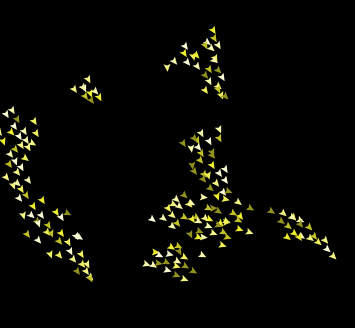
\includegraphics[scale=.66667]{images/netlogo_boidflock.png}
\caption{A boid flock moving through a two-dimensional space.}
\label{fig:netlogoboids}
\end{figure}

One of the first popular ABMs was the boid flock \cite{reynolds1987}\cite{reynolds1999sba}, in which agents move through an environment in a similar way to how birds flock.
A screen shot from NetLogo's boid implementation \cite{flocking} is shown in Figure \ref{fig:netlogoboids}.
Agents follow three simple rules:
   \begin{itemize}
      \item Move away from other agents to avoid collisions,
      \item Align to move in the same direction as nearby agents, and
      \item Move towards the central position of local flockmates.
   \end{itemize}
These simple agent-level behaviors result in the elegant flocking behavior observed from a top-down view of the system.
This system naturally lends itself to being implemented as an agent-based model because the agents act autonomously and have local interactions with only their neighbors.
The flocking behavior is emergent and therefore would be more difficult to program directly (e.g., with equation-based modeling).

Boid flocking has been used in a number of applications, such as visualizing time-varying data \cite{1382896}, clustering documents \cite{cui2006flocking}, controlling unmanned air vehicles \cite{crowther2003flocking} and art \cite{Boyd}.

Boids has remained one of my core inspirations for developing \fw.
The system is simple, yet exhibits a number of seemingly unpredictable system-level behaviors.

\subsubsection{Social Insect Behavior}

A number of different computational biology projects have aimed at modeling insect societies.
In modeling these systems, researchers are able to gain insights into how individual agent behaviors affect the system-wide emergent behavior.
These models are typically based on observations of the real insects.

An agent-based model approach has been used to model how army ants form traffic lanes \cite{couzin2003sol}.
The particular species of army ants discussed in this work form two-way highways to reduce the amount of head-on collisions while ants are searching for food and returning food.
The authors show how the turning rates and perception of the individual ants affect the efficiency of the ants.
They found that when the turning rate is too high, ants are too willing to steer off course and intersect the path of other ants.
On the other hand, when the turning rate is too low, ants will not adjust their heading to avoid head on collisions.
By tuning their model to optimize the highway performance, they reached an accurate model of the traffic flow in army ants.
The result of this research is an accurate model that describes the individual behavior of ants in a traffic situation.

With a different species of ants, researchers were able to produce an agent-based model that simulates the process of an ant colony that collectively selects a location for a new nest \cite{pratt2005agent}.
This process is interesting because an entire ant colony converges on one location, even though many of the ants only have scouted one nest site.
Agents are implemented as state machines, in which agents are either exploring for a site, assessing a site, canvassing a site or committed to a site.
In each of these phases, the agent performs different actions and at any time may reject the current site and begin exploring once again.
Over time, all ants converge on a single site as a nest.
With this model, the authors showed that a colony-level decision can be made by ants following agent-based rules.

An ABM has been developed to simulate swarming locusts \cite{buhl2006dom}.
Locusts have an interesting property in that when they are isolated, they tend to not stray from their current location.
However, when locusts are among several other locusts, they begin to ``march," travelling from one area to another, consuming everything in their path.
The authors were particularly interested in determining at what density the locusts  begin to march. By changing the number of simulated locusts in a confined space, they were able to determine at what critical density they would march.
This simulation approach is far more practical than experimenting with real locusts.
The authors suggest that their models could be used to predict when locust swarms will occur to help warn farmers to protect their crops.

These particular studies in insect behavior illustrate the need for a system like \fw.
Researchers in this field are trying to build theories of how an agent's programming can affect system-level properties.
The authors perform empirical studies to answer their research questions and test their hypotheses.
However, this approach lacks a robust mathematical understanding of the behavior correlations.
Researchers would be able to answer their questions through analytical means provided by a domain-independent approach like \fw to reduce the amount of time spent tailoring specific experiments.
More on this comparison this particular type of ABM experimentation and the approach taken by \fw is provided in Section \ref{sec:abmexp}.

\subsection{Models of Human Societies}

Although human behavior is more complicated than insect behavior, local human interactions can often be generalized to build accurate models of a subset of human society.
Most of these aim to create an accurate as possible model of the human interactions with others in order to predict some society-level behavior.

Agent-based models have been used to determine how locals would react to an incident at the Pacific Missile Range Facility (PMRF) in Hawaii \cite{zanbaka}.
The researchers used census data to represent each islander as an individual agent that either has a positive sentiment or a negative sentiment towards the missile facility.
Agents can either change its sentiment towards PMRF by either interacting with another agent that has a different sentiment or experiencing a local event.
The model simulates local events and agent interactions and displays how either positive or negative sentiment propagates throughout the island.
With this model, the authors were able to model hypothetical situations and how they effect the sentiment on the island.

EpiSims is an agent-based simulation tool that models disease outbreaks \cite{eubank2004modelling}.
It uses estimates of how diseases are transmitted and how humans interact based on census and land-use data to realistically simulate the human society.
The system simulates individuals going to work and shopping, which exposes them to the disease and exposes the disease to others.
With this system, researchers are able to predict the effectiveness of mass and targeted vaccination strategies, given a particular community.

STREETS is an agent-based model of pedestrian traffic \cite{schelhorn1999streets}.
Pedestrian traffic is affected by two major aspects: the layout of the street network and the location of attractions.
Instead of trying to analyze the behavior of the system from this data alone, STREETS simulates people to determine a number of properties of pedestrian traffic patterns.
STREETS initializes the system with a statistically accurate distribution of individuals across the environment.
Next, the agent-based model simulates the movement of agents from their arrival point to and through the urban center.
Agents visit buildings and attractions and walk between them.
Researchers use this tool to observe a top-level view that can be used to analyze the effectiveness of the urban center layout.
Hypothetical modifications to the environment can be performed in simulation to determine if it would improve the traffic situation.

In these simulations, one of the main goals is to model human society so that hypothetical changes can be made to see the changes in the behavior of the system.
This way, the researchers don't have to use real humans in social experiments.
\fw could be helpful in answering this type of research problem.
A desired system-level property could be used to determine suitable configurations by solving the reverse-mapping problem.

  % To facilitate the creation of new agent-based models, many modeling environments have been developed... (give ~1 paragraph summaries of each)


\subsection{Multi-Agent Software Frameworks}
    % Swarm
Different implementations of different multi-agent systems have many similarities.
To reduce the amount of ``boiler plate" code for each new multi-agent system, a number of unique multi-agent software frameworks have been developed in the past two decades.
In this section, I survey the most popular of these framewworks.
\fw could be configured to analyze ABMs implemented in any of these frameworks.

\subsubsection{The Swarm Simulation System}
Swarm is one of the original agent-based modeling platforms, originally developed at the Santa Fe Institute in the 1990s.
Swarm is currently supported and hosted\footnote{The Swarm website: http://www.swarm.org/} by an independent organization called the Swarm Development Group.
The developers' motivation were to enable researchers to focus less on implementation and more on actual experimentation \cite{minar1996swarm}.
To achieve this goal, they implemented a number of libraries in Objective-C and Java that aid in the creation of ``swarm" objects, the building block of a Swarm simulation.
The swarm objects manage the agents and handle the time schedulers that queue the order of agent actions.
Also, agents can be nested as hierarchies in swarm objects to allow for heterogeneous collections of agents.
Swarm is a discrete time simulation, which means time progresses as actions occur.

Unfortunately, programming in Swarm can require a significant amount of programming overhead, since the libraries are not a single integrated application \cite{kleinbreve}.
Younger software frameworks attempt to remedy this situation by providing a more cohesive library of tools.


\subsubsection{Repast}
The Recursive Porous Agent Simulation Toolkit (Repast) is a comprehensive agent-based modeling toolkit, focusing on modeling social interactions \cite{collier2003ref}.
The toolkit is freely available to download.\footnote{The Repast website: http://repast.sourceforge.net/}
Repast is fully object oriented and attempts to be as platform independent as possible, supporting programming in Java, Python, Visual Basic.Net, and more.

Repast's feature set is quite comprehensive and extensible. Repast's features are split into six modules \cite{north2006experiences}:
\begin{enumerate}
   \item The engine module -- controls the agents, environment and scheduler,
   \item The logging module -- records execution results,
   \item The interactive run module -- manages user interaction with the model,
   \item the batch run module -- allows the user to design a series of simulations to be executed in succession,
   \item the adaptive behaviors module -- provides built-in adaptive agent behaviors that use techniques such as genetic algorithms and neural networks,
   \item the domains module -- helps define environments, such as social systems, geographic information systems, and computational game theory.
\end{enumerate}
All these modules function together to provide a modular programming environment for a diverse set of multi-agent systems.
   
    % Repast
\subsubsection{Breve}
Breve is a unique 3D simulation environment that focuses on decentralized systems and artificial life \cite{kleinbreve}.
Like most other simulation environments, Breve is freely available.\footnote{Breve website:  http://www.spiderland.org/}
The authors of Breve tout that it aims to provide a platform for physically realistic 3D models.
The models simulate continuous time, and continuous space, unlike most other toolkits which model time as discrete events and have grid world environments.
In addition, some physics such as gravity and object collision resolution with friction are built-in features of every simulation.
Breve's OpenGL display engine allows for easy to implement 3D-accelerated graphics.
Users of Breve must use a custom object-oriented language called Steve.


One of the motivating applications for building Breve was Sims' (1994) evolved 3D creatures \cite{kleinbreve}.
In this project, creatures composed of several blocks and joints compete in a game to be closest to a ball.
The features of Breve naturally fit to this domain, since it has physically realistic servos and objects that can interact with one another.
Due to these features, Breve is an interesting system for modeling individual mobile agents, as well as multiple mobile agents.



\subsubsection{MASON}
    % MASON
MASON is a multi-agent simulation toolkit developed at George Mason University and is freely available.\footnote{MASON website: http://cs.gmu.edu/~eclab/projects/mason/}
MASON takes a different approach than previous multi-agent toolkits in that it strives to be minimalist and efficient for up to a million agents \cite{Luke}.
It is meant to be ran on a number of back-end computation servers in parallel, without visualization.

MASON does not have any domain-dependent tools or built-in environments like Breve or Repast, leaving most to the user to implement their environments in Java.
Although MASON is quite minimalist, it is designed to be extensible so that it can be used as a foundation for new simulation systems.

MASON simulations can be interacted with a separate visualization that binds to the simulation.
This is a different paradigm than other toolkits like NetLogo that are tightly coupled with the visualization.


\subsubsection{NetLogo}
    % Background information on NetLogo
NetLogo is a relatively new ABM system, which was started in 1999 out of Northwestern University as a derivative of StarLogo \cite{tisue2004netlogo}.
The software is free to download,\footnote{NetLogo website: http://ccl.northwestern.edu/netlogo/} but not open source.
As the name suggests, the language used by NetLogo is a derivative of Logo, a Lisp-like language.
An artifact of this language is that agents are referred to as ``turtles" in NetLogo.

NetLogo's language is tailored to the agent-based model paradigm.
Particularly, a program can change context to an individual and execute code from its point of view.
Also, populations of agents can execute these individual actions concurrently.
For example, the code to ask all the agents to move forward one unit, then turn right would be:
\begin{quote}\texttt{\small ask turtles [ fd 1 rt 90 ]}\end{quote}

The other built-in agent type is the ``patch."
Patches are organized as a grid in a two-dimensional environment that agents are confined to.
Users can interact with patches from their context, like the turtles.
Also, it is easy to retrieve turtles that are in contact with a patch and to retrieve which patch a turtle is on, from their respective contexts.
This makes turtle interactions with the environment simple to implement.

NetLogo also includes a built-in user interface and user interface editor.
The interface consists of controls, monitors and the domain visualization.
Users define controls which bind to global variables and buttons that bind to function calls.
In addition, users can add monitors and plots, which show a variable's value or plot a variable's value over time.
These are useful tools in conveying information that the domain visualization cannot.
NetLogo can be run ``headless" to facilitate parallel execution of models or to reduce run-time.

NetLogo comes with a number of extensions, most notably BehaviorSpace and HubNet.
BehaviorSpace is a tool for designing a series of systematic experiments with different system configuration parameters.
BehaviorSpace performs a user-defined measurement value after each individual execution and reports the result to a data set in the form of a spreadsheet.
HubNet is a server/client tool that allows several users of a system to interact with a NetLogo ABM at the same time, which is useful for classroom instruction.

NetLogo can be interacted with from an external Java API.
A NetLogo ``workspace" is instantiated as an object and can be used to send commands and query current variable values.
This is useful for an number of tasks.
First, sometimes NetLogo's language is not expressive enough and some may find programming in Java more familiar.
In addition, external Java libraries (such as machine learning libraries) can be used without modification by integrating with NetLogo from its Java API.
Also, a sequential experiment system can be implemented in Java if a user would like to run experiments without BehaviorSpace.

An extensive model library with over 140 sample models is bundled with the NetLogo distribution.
These already existing models serve as excellent examples for new models as well as starting points for modified models.
Most of the domains discussed later in this dissertation are from this model library.

NetLogo is my ABM system of choice for this dissertation research for a number of reasons.
First, NetLogo's learning curve is surprisingly short.
From personal experience, a new user can learn to write a domain similar to the Wolf Sheep Predation model in less than a couple hours.
In addition, the documentation\footnote{The NetLogo documentation is available at http://ccl.northwestern.edu/netlogo/docs/} is well organized and detailed.
Second, the model library provides several models that are interesting and easy to work with.
Since each of these models are implemented in NetLogo, I was able to implement \fw so that it interacts with each ABM in a similar way.
Other multi-agent system toolkits provide more flexibility in implementation, which would make identifying agent-level control parameters and system-level properties more difficult.
Third, although NetLogo's platform is well contained, the interactions possible with the Java API make almost anything possible.
I was able to implement my framework as an external modular application that interfaces with NetLogo, instead of a built-in system dependent tool.
This makes my research easily extensible to other ABM systems in the future.

  % NetLogo - used by this research
    % Concept - based off logo, 2d domain of patches, agents are ''turtles''
    % Agents are asked to perform actions from their context. e.g., ask turtles [ fd 1 ]
    % Plotting and monitors
    % BehaviorSpace extension for sampling
    % Java APIs


\section{Regression}
Regression is an integral part of this dissertation research, as it is the foundation of solving the forward- and reverse-mapping problems.
  % The reason for regression: we have independent and independent real-valued variables.
Regression techniques are used to predict values of dependent variables, given values of the independent variables.
The typical approach is to use a model developed from a sample training set to infer new values that of configurations that have not been sampled.
Also, regression can be used to smooth the natural error in sampling.

Linear regression is perhaps the simplest form of regression. It fits a line to represent the correlation between one independent variable with one dependent variable, taking the form of:
\[\mathrm{y} = \mathrm{x} + b.\]
There exists a closed-form solution to determine $m$ and $b$ in order to minimize the sum of squares between the training data and the curve.

Unfortunately, linear regression is limited in that it only models linear relationships, and is not able to model nonlinear ones, such as rhythmic oscillations, or quadratic correlations.
Two paths are generally taken to address this concern.
The first is to use the kernel trick \cite{muller2001introduction} to map nonlinear data to be linear, but higher dimensional.
Then, once the data is projected into a space in which it is linear, linear methods (e.g., linear regression, perceptrons \cite{minsky19882perceptrons}, or support vector regression\cite{smola2004tsv}) can be used.

% Regression
   % Give definition of the regression problem
The second approach is to use nonlinear methods, which relax linear regression to learning a function $f: \mathbb{R}^n \rightarrow \mathbb{R}$ that satisfies the following equality:
\[y_i = f(\mathbf x_i) + \varepsilon_i.\]
In this equation, $y_i$ is a dependent variable and $\mathbf x_i$ is the vector of independent variables associated with $y_i$.
Also, there is an assumption of some normally distributed and independent error with each point, denoted by $\varepsilon_i$.
The process of \textit{nonparametric} regression is to estimate this function directly \cite{fox2002r}.

Alternatively, a \textit{parametric} regression model has the form of the function $f(\cdot)$  relatively fixed.
Instead of learning $f(\cdot)$ directly, a vector of model parameters $\mathbf \beta$ are optimized to fit the data \cite{fox2002r}:
\[y_i = f(\mathbf \beta, \mathbf x) + \varepsilon_i.\]
For example, $f(\cdot)$ could model two-dimensional sinusoidal data with the model:
\[f(\mathbf \beta, (x_1, x_2)) = \beta_1 + \beta_2 \sin (x_1 - \beta_3) + \beta_4 \sin (x_2 - \beta_5)\]
Typically, the value of the least squares metric is minimized to fit the curve to the data.

  % What I need in a regression algorithm: can model nonlinear behaviors that are difficult to apply a model to and works in many dimensions; needs to build relatively smooth models for the inverted regression to be smooth.
While developing the \framework, I needed regression algorithms that satisfied a number of properties.
The regression algorithm should scale well with dimensionality, since agent-based model behavior spaces (i.e., the space of agent-level parameters and system-level properties) are typically highly dimensional.
I also needed algorithms that could model nonlinear correlations, since behavior spaces are expansive and rarely maintain linearity throughout the entire space.
However, in the ABMs I have experimented with, all spaces are very smooth locally.
That is, there is little variance in values between nearby locations in the behavior space.
Even in the situation where there is variance, the error is typically evenly distributed and cancels out if the same configuration is sampled a number of times.
Therefore, nonlinear parametric regression can fit to the overall behavior space, without having to worry about fine grained variations in the data.
Also, the mappings built by the regression models should be smooth.
This is important for the tractability of finding the reverse mapping, since bumpy surfaces will naturally yield more intersections than smooth ones.
Therefore, regression methods that smooth the data, such as LOESS, are effective in this situation.

\textit{[\textbf{TODO}: an image showing graphs of the fires, boids, and sheep/wolf predation behavior spaces (need to make wolf/sheep data set to do this)]}

In the course of testing \fw, I used four regression techniques: k-nearest neighbor, LOESS, least-squares nonlinear regression, and Multilinear Interpolation.

  % Figure of Fires domain, boids domain, wolf/sheep predation domain behavior graphs
  % So far, I have implemented the following regression algorithms to work with \fw: K-Nearest Neighbor, LOESS (Locally weighted scatterplot smoothing, least-squares Non-Linear Regression, Multilinear Interpolation
\subsection{K-Nearest Neighbor Regression}
  % K-Nearest Neighbor Regression
    % Concept - Take k-nearest neighbors and average them
K-nearest neighbor (KNN), in general, is the process of selecting the $k$ nearest points to some point $\mathbf x$.
These points can then be used for classification or regression.
In the simplest case, each neighbor's $y$ value is averaged to infer a value $\hat y$ for the given point $\mathbf x$.
KNN is easy to implement and accurate with large data sets.
Accuracy of this regression can be improved by weighting points by distance or by using a secondary regression algorithm (e.g., linear regression) on the neighbors.

    % The role of KNN - easy to implement, accurate with large data sets
We use KNN in our results as a baseline, since it is easy to implement and accurate.
In addition, it is nonparametric, which makes it agnostic the the shape of the behavior space.
Therefore, KNN requires little to no configuration or tailoring to a particular domain.

    % Slow with large data sets because of all the distance calculations needed.
      % Can be sped up with advanced nearest neighbor search, such as a kd-tree or local sensitivity hashing.
However, when implemented naively, the run-time scales linearly with the size of the data set because the process of finding the nearest neighbors requires a scan of all data points.
This search time can be reduced with the implementation of faster searching techniques, such as locality sensitive hashing \cite{gionis1999similarity}, among other methods.
Even with faster neighbor locating techniques, some sort of search is required for each query to KNN.

The spaces generated by KNN are not continuous (particularly if the neighbors are not weighted).
This is because similar points will have the same neighbors and, in effect, have the same predicted value.
There are separations in which on one side the k-nearest neighbors will include a particular data point, meanwhile on the other side it will not.
At this separation, a noncontinuous jump will occur in predicted values.
This can be a problem for solving the reverse-mapping problem because the intersection between hyperplanes generated by KNN will not intersect smoothly.
This can be remedied by using KNN in conjunction with multilinear interpolation.
      
\subsection{Robust Locally Weighted Regression and Smoothing Scatterplots (LOESS)}


    % Advantages: nonparametric (useful for my domains), 
    % Role in \fw : accurate and nonparametric. Conceptually, if we sample infinitely with LOESS, we will get a very smooth graph (which makes it nice for inverted regression).
Robust Locally Weighted Regression and Smoothing Scatterplots (LOESS) is a mature nonparametric regression technique for fitting curves to data   \cite{cleveland1979robust}\cite{cleveland1988locally}.
Similar to k-nearest neighbor, LOESS uses local points to infer values of new data points.
LOESS also iteratively smooths the regression curve, allowing for variable magnitudes of smoothing.
This is important for particularly noisy data sets.
The role of LOESS in the testing of \fw is that it is more robust than KNN, yet still nonparametric.

    % Concept - take some subset of neighbors, weight them, and then perform linear regression on them
Abstractly, LOESS fits a new $\hat y_i$ to every $\mathbf x_i$ to replace the original noisy $y_i$.
Then, LOESS iteratively smooths each $\hat y_i$ to reduce variability.
Specifically, LOESS follows the following steps:
\begin{enumerate}
   \item Initialization step -- for each $\mathbf x_i$, weight all other points $x_j$, where $j = 1...n$, based on a weighting function $W(\mathbf x_i, \mathbf x_j)$. $W$ weights closer points higher. Perform weighted linear regression to infer $\hat y_i$.
   \item Smoothing step -- For each $\mathbf x_i$, weight all other points based on $w_i$, as well as a new weight function $\delta$, which returns magnitude inversely proportional to $y_i - \hat y_i$ (i.e., the larger the distance, the lesser the weight). Perform weighted linear regression to infer $\hat y_i'$.
   \item Set each $\hat y_i$ to $\hat y_i'$.
   \item Repeat the the smoothing step as many times as necessary.
\end{enumerate}
Values in between $\mathbf x$s can be now be interpolated.

    % Role of the smoothing parameter -- how much data is used to fit each polynomial
LOESS can be customized in a number of ways.
The different weighting functions can be changed to change the amount of influence other points give to the linear regression step.
Typically, these weighting functions have a ``smoothing" parameter, which increases the influence of further away points, effectively reducing the strong influence of local points.
Adjusting the smoothing parameter is important because if it is too low, the regression curve will be erratic (i.e., overfit), meanwhile, if the smoothing parameter is too high, some features of the curve may be eliminated.

  % LOESS
    % Weight function weights points by distance -- most common function is the tri-cube function
LOESS is relatively computationally expensive in comparison to other approaches.
This is because  weights are applied and points are readjusted iteratively a number of times.
However, the model can be built offline and then stored.
Once the $\hat y_i$ values are inferred, they can be used to interpolate new points (similar to multilinear regression) in response to queries.
This provides a quick response time to users wanting to infer $\hat y$ values.
This fits one of the design criteria of \fw: the regression algorithm should be fast for the user.

The \textit{R} statistical package\footnote{R website: http://www.r-project.org/} has a built in LOESS function.

\subsection{Nonlinear Regression}

Nonlinear regression (NLR) is a parametric approach to regression.
  % NonLinear Regression
    % Concept - take a model of the data, optimize the parameters to minimize least squares.
With this approach, a parametric model is provided by the user that represents the relationships in the data, in general.
This is typically done with some sort of intuition on behalf of the user.
For example, the data may appear sinusoidal or quadratic, in which case a model involving sine curves or quadratic polynomials, respectively, would be appropriate.
    % Accuracy is largely dependent on the model
Similarly to how linear regression will not model nonlinear relationships well, certain nonlinear models will not model other nonlinear relationships.
Therefore, accuracy is largely dependent on the selection of the correct model.

Optimization techniques, such as Gauss-Newton or Levenberg-Marquardt \cite{mor1977levenberg}, are used to adjust nonlinear model parameters in order to minimize the least squares metric \cite{gallant1975nonlinear}.
These processes iteratively move models towards the best fit to the data.

Nonlinear regression is of particular interest in my research because it is analytically invertible, since trained NLR models are already in the form of a function.
Unfortunately, since NLR is parametric, it requires a significant amount of configuration between different target domains.

    % Limited (for example, had trouble modeling the simple sigmoid looking thing from the fires domain).
    % Advantage: fast to query
    % Role in \fw: algebraically invertible (more in chapter: reverse mapping)




\subsection{Multilinear Interpolation}

  % Multilinear Interpolation
    % Concept - given corner points of a hypercube (knots), interpolate some point inside of it with linear interpolation; interpolate dimension my dimension until the point is reached.
Multilinear interpolation is a dynamic approach that uses multi-dimensional interpolation between ``knots" to generate a smooth surface across a space of any dimension \cite{davies1997multidimensional}.
Knots are sampled data points, scattered across the behavior space in a regular fashion such that the knots, when connected, form hypercubes.
When a point $\mathbf x$ is queried, multidimensional interpolation is performed using the corners of the hypercube to infer the value of $\hat y$.

    % Downside - sampling needs to be systematic: remedy- use another regression algorithm to build the knots. This has the benefit of being faster than other approaches (the interpolation is fast, the regression may be slow, and the knots can be built ahead of time)
The major downside to multilinear interpolation is that the sampling needs to be systematic and evenly spaced.
To remedy this situation, another regression algorithm is used to compile a set of evenly spaced points.
These evenly spaced inferred points area then passed to a traditional multilinear interpolation approach.

In this dissertation, I typically use multilinear interpolation as a supplement to  other regression approaches.
Any irregularly sampled data set can be converted to a evenly spaced one by inferring knot locations with another regression technique.
Once this intermediary inferred data set is in place, standard multilinear interpolation can be used.

    % Faster than some of its counterparts
    % builds smooth mappings of multi-dimensional spaces

%\section{Inverting Regression}
% How does inverting regression fit into \fw? We invert the forward mapping to solve the reverse-mapping problem.
% Our two major approaches to this are optimization and plane intersection.
% More approaches are possible and are discussed in Chapter X: The Reverse-Mapping problem, but require limited amount of background information.


\section{Surface Intersection}
    % Plane Intersection
       % What does plane intersection do? it takes two hyperplanes and returns the intersection.
The surface-to-surface intersection (SSI) problem is the problem of finding the intersection between two surfaces.
This is a difficult problem due to the variety of shapes and configurations of high-dimensional spaces.
Surface-to-surface intersection algorithms for solving these problems can take a number of forms:
lattice evolution methods, marching methods, subdivision methods, and analytic methods \cite{patrikalakis1993surface}.

TODO: [Give specific examples of SSI algorithms; a more comprehensive literature survey of SSI is needed] \cite{huber}


   % How we use plane intersection: The solution to the reverse-mapping problem is the intersection of the forward mapping and the plane representing the desired behavior.
   % Give example
   % Figure example
SSI serves an important purpose in solving the reverse-mapping problem.
First, SSI is used to find the space of configurations that would satisfy a desired system parameter.
To apply SSI approaches, we frame the problem of solving for $f^{-1}(y_k) = \hat{\mathbf x}_k$ (i.e., find $\hat{\mathbf x}_k$, given $y_k$) as an SSI problem.
This is done by finding the intersection $\vec{w} : \vec{u} \bigcap \vec{v}$ between the surfaces $\vec{u}: y = y_k$ and $\vec{v}: y = f(\mathbf x)$.
In this case, $f$ is the forward mapping space.
The surface $\vec{w}$ can be used to extract valid configurations that will produce the behavior $\hat y$.
This approach can be expanded to satisfy a number of system-level properties at once.
For example, in the Wolf Sheep Predation model, a user might want to find configurations of a system that typically averages 100 sheep and 80 wolves.
Intricacies and extensions to this approach are discussed in Chapter \ref{ReverseMapping}: The Reverse-Mapping Problem.








   % Benefits of this approach: gives a space that represents the intersection, instead of just one point.
   % Slow

%\subsection{Optimization}
    % Optimization
       % Minimize the distance from the result of the forward mapping to the actual result
       % Stochastic Hill Climbing
           % very simple, works well in domains with not many local minima
       % Other possible approaches:
           % Gradient ascent, genetic algorithms

   % How we use optimization: Try to minimize the distance between the produced system-level property and the desired system-level property by adjusting the agent-level parameters.

   % Benefits: fast
   % bad: only finds one solution

